\documentclass[12pt]{article}
\usepackage[utf8]{inputenc}
\usepackage{float}
\usepackage{amsmath}
\usepackage{graphicx}
\usepackage{verbatim}

\usepackage{tikz}
\usepackage[hmargin=3cm,vmargin=6.0cm]{geometry}
\topmargin=-2cm
\addtolength{\textheight}{6.5cm}
\addtolength{\textwidth}{2.0cm}
\setlength{\oddsidemargin}{0.0cm}
\setlength{\evensidemargin}{0.0cm}
\usepackage{indentfirst}
\usepackage{amsfonts}

\begin{document}

\section*{Student Information}

Name : Mithat Can Timurcan\\

ID : 2581064


\section*{Answer 1}
\subsection*{a)} 
\begin{itemize}
    \item In order to determine the size of our Monte Carlo simulation, we can use Normal approximation witht the values $\alpha = 0.01$ and $\epsilon = 0.02$.
    \item However, since we don't have an "intelligent guess" estimator $p^*$, we are going to use the following:
    \begin{equation*}
        \begin{split}
            N \geq 0.25 \cdot { \left(\frac{z_{\alpha/2} }{\epsilon}\right) }^2 = 0.25 \cdot { \left(\frac{2.575}{0.02}\right) }^2 = 4144.14 \approx 4144
        \end{split}
    \end{equation*}
    \item Therefore, we see that the size of our simulation $N$ should be greater than 4144. We can pick $N = 4145$ for our simulation.
\end{itemize}

\subsection*{b)}
\begin{itemize}
    \item Since we have the information that the weight of each automobile is a Gamma distributed random variable in kilograms with $\alpha = 120$
    and $\lambda = 0.1$, we can use the expected value formula for Gamma distribution:
    \begin{equation*}
        \begin{split}
            \textbf{E}(X) = \frac{\alpha}{\lambda} = \frac{120}{0.1} = 1200 
        \end{split}
    \end{equation*}
    \item Similarly, since the weight of each is a Gamma distributed random variable in kilograms with $\alpha = 14$
    and $\lambda = 0.001$, we can use the expected value formula for Gamma distribution:
    \begin{equation*}
        \begin{split}
            \textbf{E}(X) = \frac{\alpha}{\lambda} = \frac{14}{0.001} = 14000
        \end{split}
    \end{equation*}
    \item Since the weight of an automobile and the number of automobiles passing through a bridge are independent events, we can just multiply the expected values:
    \begin{equation*}
        \begin{split}
            \textbf{E}(XY) = \textbf{E}(X) \cdot \textbf{E}(Y) = 1200 \cdot 60 = 72000 \ \text{where} \ \textbf{E}(Y) = \lambda_A = 60
        \end{split}
    \end{equation*}
    \item Similarly, the weight of a truck and the number of trucks passing through a bridge are independent events, we can just multiply the expected values:
    \begin{equation*}
        \begin{split}
            \textbf{E}(XY) = \textbf{E}(X) \cdot \textbf{E}(Y) = 14000 \cdot 12 = 168000 \ \text{where} \ \textbf{E}(Y) = \lambda_T = 12
        \end{split}
    \end{equation*}
\end{itemize}

\section*{Answer 2}

\begin{verbatim}
    N = 4145;
    lambdaA = 60;  % number of automobiles
    lambdaT = 12;  % number of trucks
    
    alphaA = 120; lambdaA_2 = 0.1; % Gamma distribution lambda
    alphaT = 14; lambdaT_2 = 0.001;
    
    TotalWeight = zeros(N, 1);
    for k = 1:N
      % first generate the number of passed vehicles for each type from Poisson
      numA = 0;
      numT = 0;
    
      % number of automobiles
      U = rand;
      F = exp(-lambdaA);
      while (U >= F)
        numA = numA + 1;
        F = F + exp(-lambdaA) * lambdaA ^ numA/gamma(numA + 1);
      end
    
      % number of trucks
      U = rand;
      F = exp(-lambdaT);
      while (U >= F)
        numT = numT + 1;
        F = F + exp(-lambdaT) * lambdaT ^ numT/gamma(numT + 1);
      end
    
      weight = 0; % total weight of vehicles for this run
    
      % calculate the total weight of automobiles
      weightA = 0;
      for j=1:numA
        weightA = weightA + sum(-1/lambdaA_2 * log(rand(alphaA, 1)));
      end
    
      % calculate the total weight of trucks
      weightT = 0;
      for j=1:numT
        weightT = weightT + sum(-1/lambdaT_2 * log(rand(alphaT, 1)));
      end
    
      weight = weightA + weightT;
      TotalWeight(k) = weight;
    end
    
    p_est = mean(TotalWeight>250000);
    expectedWeight = mean(TotalWeight);
    stdWeight = std(TotalWeight);
    
    fprintf('Estimated probability = %f\n', p_est);
    fprintf('Expected weight = %f\n', expectedWeight);
    fprintf('Standard deviation = %f\n', stdWeight);
    \end{verbatim}
\begin{itemize}
    \item I've used JDoodle online compiler to run my code and got the following results:
\end{itemize}
\begin{figure}[H]
    \centering
    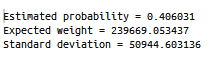
\includegraphics[width=0.35\textwidth]{code_and_output/image.png}
    \caption{Outputs of our simulation.}
    \label{fig:example_b}
\end{figure}
\begin{itemize}
    \item We got a standard deviation $X$ of 50944 kilograms in our simulation. This is a high variability compared to our expected value of 239669 kilograms which means that individual $X$ values may differ from the expected true value of $X$. We can say that our accuracy is not that high.
    \item For the limiting value of $\lambda_T$, I've tested the values that might make the probability of bridge’s collapse close to 0.1 which are 8 and 9:
\end{itemize}
\begin{figure}[H]
    \centering
    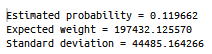
\includegraphics[width=0.35\textwidth]{code_and_output/image2.png}
    \caption{Output of our simulation when $\lambda_T = 9$.}
    \label{fig:example_b}
\end{figure}
\begin{figure}[H]
    \centering
    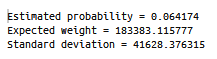
\includegraphics[width=0.35\textwidth]{code_and_output/image3.png}
    \caption{Output of our simulation when $\lambda_T = 8$.}
    \label{fig:example_b}
\end{figure}
\begin{itemize}
    \item It can be seen from the outputs, when $\lambda_T \geq 9$ the probability of bridge’s collapse is greater than 0.1. Therefore, we can say that our limiting value is $\lambda_T = 8$.
\end{itemize}
\end{document}
